\section{Jurnal Faza 1}

\setlength\parindent{24pt}
% ============================================= Cerintele rezolvate====================================== 
\subsection{Cerințele rezolvate}
% enuntul intrebarii
\hspace{\parindent}
Proiectul dezvoltat în cadrul laboratorului de Administrarea Sistemelor de Operare presupune realizarea unui web-site minimal cu simularea lansării acestuia în producție. Principalul scop al acestui proiect  este acela de familiarizare cu tehnologiile folosite și lansarea lui in producție. \newline
\par Dezvoltarea site-ului se va realiza cu ajutorul framework-ului Django (bazat pe limbajul de programare Python), iar în primă fază cerințele s-au concetrat asupra instalării și preagtirii mediului de dezvoltare a aplicației. De asemenea, la finalul acestei etape s-a dorit crearea unui site minimalist pe baza comenzilor oferite de biblioteca Django instalată pentru Python și crearea interfeței de administrotor (un superuser).

\subsection{Modul de rezolvare}
\hspace{\parindent}În această subsecțiune sunt cuprinși pașii efectuați pentru rezolvarea cerințelor propuse în această fază a proiectului. Aceștia vor fi descriși în ordinea efectuării lor și se va prezenta necesitatea acestora în finalizarea cerințelor cerute 

\subsubsection{Mediul de dezvoltare a aplicației}
\hspace{\parindent}
Mediul local de dezvoltare a aplicatiei este pe un sistem de operare linux. Sistemul de operare al calculatorului personal este Linux Mint 20.3 Cinnamon, versiunea Cinnamon 5.2.7. Principalele avantaje ale unui sitem de operare linux se referă la faptul că e un program de tip open-source ce are o securitate performantă, e stabil, suportă majoritatea limbajelor de programare și are un management al fisierelor performant, suportând fișiere de aproape orice format. \par
Versiunea de python pe care o am este 3.9.12. Pentru crearea site-ului minimalist a fost nevoie de instalarea bibliotecii Django. S-a instalat un official release pentru Django cu ajutorul package installer-ului \textbf{pip}. Aceasta este printre principalele metode recomandate pe site-ul oficial al framework-ului 
\begin{minted}{bash}
  $ python -m pip install Django
\end{minted}

\par
Django este un framework folosit pentru dezvoltarea site-urilor web ce urmează un model arhitectural de tipul Model-View-Controller. La crearea unui proiect Django se creează principala structură a site-ului cu separarea functionalitățiilor pe pachete specializate. Un alt avantaj al framework-ului este acela că oferă un panou administrativ, astfel un user cu rol de superuser in aplicație poate accesa acest panou de administrare a aplicatiei și poate crea, citi sau actualiza informațiile cuprinse în baza de date. O cerință din cadrul acestei faze a proiectului se refera la activarea acestui panou administrativ și crearea unui super user cu un username și parolă care poată să acceseze ulterior pagina de admin. Versiunea de Django actuală este 4.1.2 .

\subsubsection{Crearea structurii initiale a site-ului}
\hspace{\parindent} Pentru crearea structurii initiale a site-ului s-a rulat următoarea comandă. În urma rulării comenzii s-a creat un fișier \textit{manage.py} și un folder în care se regăsesc principalele fișiere de configurare ale aplicației web. 
\begin{minted}{bash}
    $ django-admin startproject claudiu_first_site
\end{minted}

Fișierele create conțin informații despre configurarile și setăriile proiectului in ceea ce privește aplicațiile pe care le conține și conexiunea la baza de date (\textbf{settings.py}). De asemenea, cuprinsul cu toate rutele url ale aplicației sunt incluse intr-un fișier denumit \textbf{urls.py}. De asemenea, se mai creează un fișier important (\textit{manage.py}) ce reprezintă un utilitar pentru linia de comanda la pornirea server-ului local al aplicației. \par
Pornirea server-ului local de test al site-ului se realizează prin rularea comenzii de mai jos si se poate accesa la portul default 8000. Acest port se poate de asemenea modifica din fisierul de settings.
\begin{minted}{bash}
    $ python manage.py runserver
\end{minted}

\subsubsection{Crearea unei applicatii pentru proiect}
\hspace{\parindent} Am creat prima aplicatie din cadrul proiectului pe care am denumit-o conform tutorialului \textit{aso}. Pentru această aplicație s-a creat un view de \textit{"Hello world"} care e accesibil la URL-ul \textit{localhost:8000/aso/}. Am creat in interiorul folder-ului specific aplicației nou  create un fisier denumit \textit{urls.py}, unde am definit pentru un urlpattern ce functie din cadrul view-urilor definite să se apeleze în momentul accesării lui. Asftel, pentru un context '' în cadrul aplicatiei \textbf{aso} se va apela view-ul de Hello World (vezi imagine 1). 
\begin{minted}{bash}
    -crearea aplicatiei aso---
    $ python manage.py startapp aso
\end{minted}

\begin{figure}[htp]
    \centering
    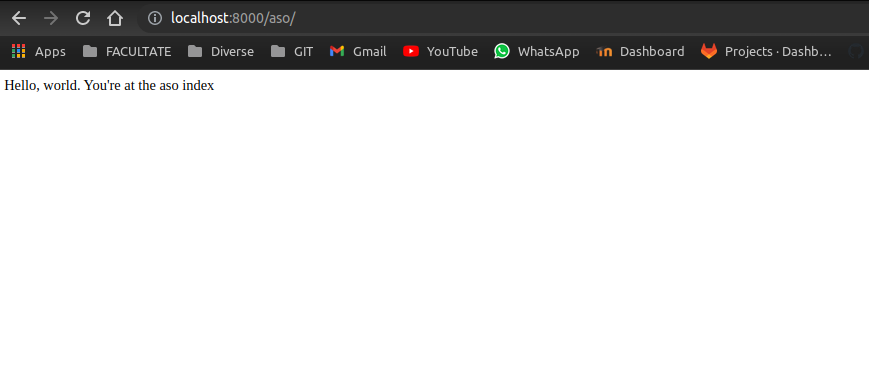
\includegraphics[width=10cm]{text/images/helloworld.png}
    \caption{Hello world aso app}
    \label{fig:galaxy}
\end{figure}

\subsubsection{Crearea unui super user}
Am creat prin intermediul comenzii de mai jos un super user și am accesat panoul administrativ prin intermediul logarii cu acest user. 
\begin{minted}{bash}
    $ python manage.py createsuperuser
\end{minted}
% descrieti aici orice fel de probleme ati intampinat in timpul rezolvarii acestui task si modul cum in care le-ati solutionat
\vspace{0.75cm}

\subsection{Probleme întâlnite și modul de rezolvare}
\hspace{\parindent} Nu am întâmpinat probleme, iar procesul de creare a minisite-ului a fost ușor de urmărit. 
\subsection{Concluzii}
\hspace{\parindent} Ceea ce apreciez la un proiect creat prin intermediul framework-ului Django este faptul că îți impune de la început să îți structurezi proiectul după modelul MVC. Respectarea acestui template va oferi un grad ridicat de reutilizare a codului.

\subsection{References}
\url{https://docs.djangoproject.com/en/3.2/intro/tutorial01/}
